\index{Modeling!Add Elements}
\index{Add Elements to Model}

Once you have created a modeling \gdproject{} \bxpref{TasksMBTCreateProject} and created a model \bxpref{TasksMBTCreateModel} or imported one \bxpref{TasksMBTImport}, you can start working on your model. 

\bxtipp{We recommend validating your model frequently \bxpref{TasksMBTValidate}.}
\begin{enumerate}
\item If the \gdmodeleditor{} is not open, open it by double-clicking on the model you want to work on in the \gdnavview{}. 
\item In the palette on the right-hand side of the \gdmodeleditor{}, you will see the four \bxname{nodes} and the one \bxname{connector} that you can use to create your models. These are:
\begin{description}
\item [\gdcase{}:]{These are the building blocks of your test. When you generate your model, they become normal \jb{} \gdcases{} \bxpref{WorkingWithTestCases}. Use \gdcases{} to model actions or sequences of actions in your \gdaut{}. }
\item [\gdcase{} reference:]{As with any \jb{} test, \gdcases{} can be reused in other \gdcases{}. Add \gdcase{} references to the \bxname{reused \gdcase{}} area in a \gdcase{} node to indicate that you want to reference a \gdcase{} here. You will need to add a connector line between the \gdcase{} reference and the referencing \gdcase{} in your model.} 
\item [Parameter:]{\gdcases{} can have parameters for data that this \gdcase{} will reference. You can add parameters to the \bxname{parameter} area in \gdcase{} nodes. Adding parameters in this way is the equivalent of referencing parameters in the specification perspective using the equals sign \bxpref{TasksTestdataReferences}.}
\item [Category:]{You can group the \gdcases{} in your model into categories. These will later be generated into \jb{} categories in the \gdtestcasebrowser{} \bxpref{TasksTCCats}. Use categories to organize your \gdcases{}.}
\item [Define reused \gdcase{}:]{Once you have added a \gdcase{} reference to a \gdcase{} in your model, you must use this connector to show which \gdcase{} the reference reuses. Click and drag the connector from the \gdcase{} reference to the \gdcase{} it reuses.}
\end{description}
\end{enumerate}

\subsubsection{Adding \gdcases{} to the model}
To add a \gdcase{} to the model:
\begin{enumerate}
\item Click once on the \gdcase{} node in the palette then click in the \gdmodeleditor{} to place the \gdcase{}. The \gdcase{} appears on the canvas. 
\bxtipp{You do not need to drag and drop the elements from the palette.}
\item Enter a name for the \gdcase{} either directly in the model, or in the \gdpropview{} in the modeling perspective. 
\end{enumerate}

\subsubsection{Adding parameters to \gdcases{} in the model}
To add parameters to a \gdcase{} in the model:
\begin{enumerate}
\item Click once on the \bxname{Parameter} node in the palette.
\item Click in the \bxname{parameter} area of the \gdcase{} you want to add the parameter to in the \gdmodeleditor{}.  The parameter appears in the \gdcase{}. 
\item Name the parameter either directly in the model, or in the \gdpropview{} in the modeling perspective. 
\item In the \gdpropview{}, select the type of parameter: \bxname{String, Integer, Boolean} or \bxname{Variable}.
\end{enumerate}

\subsubsection{Adding referenced \gdcases{} and connections in the model}
To reference a \gdcase{} in the model:
\begin{enumerate}
\item Click once on the \bxname{\gdcase{} Reference} node in the palette.
\item Click once in the \bxname{reused \gdcase{}} area of the \gdcase{} you want to add the \gdcase{} reference to in the model. The \gdcase{} reference appears in the \gdcase{}. 
\item Click once on the \bxname{Define Reused \gdcase{}} node in the palette. 
\item In the canvas, drag the connection from the reused \gdcase{} you just added to the actual \gdcase{} you want to reference. The name of the \gdcase{} you are referencing will automatically appear in the referenced \gdcase{} (\bxfigref{ModelReusedTCs}). 
\end{enumerate}

\begin{figure}[h]
\begin{center}
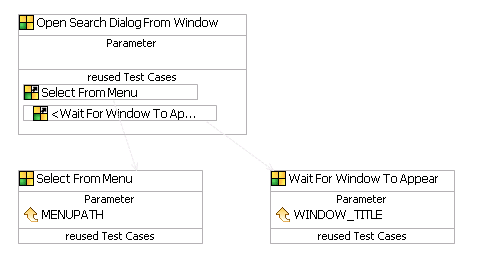
\includegraphics{Tasks/Modelling/PS/Model_ReusedTCs}
\caption{Model showing referenced Test Cases}
\label{ModelReusedTCs}
\end{center}
\end{figure} 

\subsubsection{Adding categories to the model}
To add a category to the model:
\begin{enumerate}
\item Click once on the \bxname{Category} node in the palette and then click in the \gdmodeleditor{} to place the category. The category appears on the canvas. 
\item Enter a name for the  category, either directly in the model or in the \gdpropview{} in the modeling perspective.  
\item To add items already on the canvas to a category, drag the item and drop it into the category area. 
\item To add items directly to a category, select the item from the palette and click into the category to place it here. 
\bxtipp{When the category is selected, you can see a small arrow in the left-hand corner. This arrow must be pointing down to be able to add items to the category.}
\end{enumerate}
